\documentclass[a4paper, 11pt]{article}
\usepackage{graphicx}
\usepackage{algorithm}
\usepackage{algpseudocode}
\usepackage{amsmath}
\usepackage{listings}
\usepackage[margin=0.8in]{geometry}

\title { Visual Analytics\\ \bigskip \large Propostal: Mobile applications}
\date{21 April 2020}
\author{Silvio Dei Giudici 1708962 \\ Marco Morella 1693765}

\begin{document}

\maketitle

\section{General Idea}
The increasingly cheap mobile technology has induced in the latest years an exponential growth in the mobile application market, to the point that any user has a selection of applications and tools available to download which is so wide and confusing that picking out the fittest one is often a challenge on its own.\\
Due to the particular nature of this problem, the standard app store is often not helpful thus we aim to create a visualization tool where the user can analyze the information given by the store and filter out applications to find the best one dinamically.\\
We will use a dataset containing ten thousand application with all possible information given by the play store, retrieved by web-scraping the browser instance of Google Play Store, made by an user on kaggle.com.\\
\section{Dataset}
As we said before the dataset contains 10 000 applications, with 13 features which will be analyzed in the following.
\begin{itemize}
\item \textbf{Application name}.
\item \textbf{Category}: one between 34 possible categories in which the Play Store divides its applications, some of which are Game, Business, Communication and so on.
\item \textbf{Rating}: value between 1.0 and 5.0, based on the average review received by the app.
\item \textbf{Reviews}: number of reviews received by the app.
\item \textbf{Size}: size of the app.
\item \textbf{Installs}: number of times the app has been installed by users.
\item \textbf{Type}: whether of not the app is a paid or free one.
\item \textbf{Price}: self-explaining, does not include in-app purchase.
\item \textbf{Content rating}: age group the app is targeted for.
\item \textbf{Genres}: list of genres the app belongs to, e.g. Health, Tools, Entertainment and so on.
\item \textbf{Last updated}: date of last update on the play store for the app.
\item \textbf{Android version}: minimum required version to run the application.
\end{itemize}
The database contained one more feature which was deemed not useful for analysis which is \textbf{Current version}. Since every developer uses a different(personal) way to denote the released versions it wouldn't have made much sense in a visualization.
\section{MDS}

\section{Visual Project}
In the following we will go over each visualization we want to implement through D3.js, an initial mock-up can be seen in the last page of the proposal.
\begin{itemize}
\item \textbf{Parallel coordinates chart} containing most of the features which should help the user see the general statistic related to the apps he's currenting filtering for.
\item \textbf{Three boxplots} to let the user analyze the distribution over Size, Review and Rate.
\item \textbf{One scatter plot} showing the applications using MDS analysis.
\item \textbf{One horizontal histogram} showing the distribution of samples over the categories.
\item \textbf{One histogram} for the distribution of samples over content rating.
\item \textbf{One histogram} over the occurences of minimum android version required. In order to have a clearer vision of the distribution without having too many separate sections we stacked the different updates of the main version: all y.x stay in the column of y.0.
\end{itemize}
Furthermore we will put a list(or table) of applications fitting in the user filtering. Obviously since this is a proposal made before starting the work we may find out some other visualizations/interaction we may want to implement to improve our visualizations.
\section{User interactions}
In our visualization the user will be able to select one or more value from each parallel coordintes chart to put them in the filter, anything not coherent with those values will be filtered out of the dataset thus reflecting on all other visualizations.\\
The same thing will be doable on all three histograms if any of the column is clicked, else if it the user only hovers over them they will be highlighted on the other graphs.\\
The only items which won't be interactable for the user will be the MDS scatter plot and the boxplots and they will only reflect the changes created by interacting with the previously defined visualizations. \\
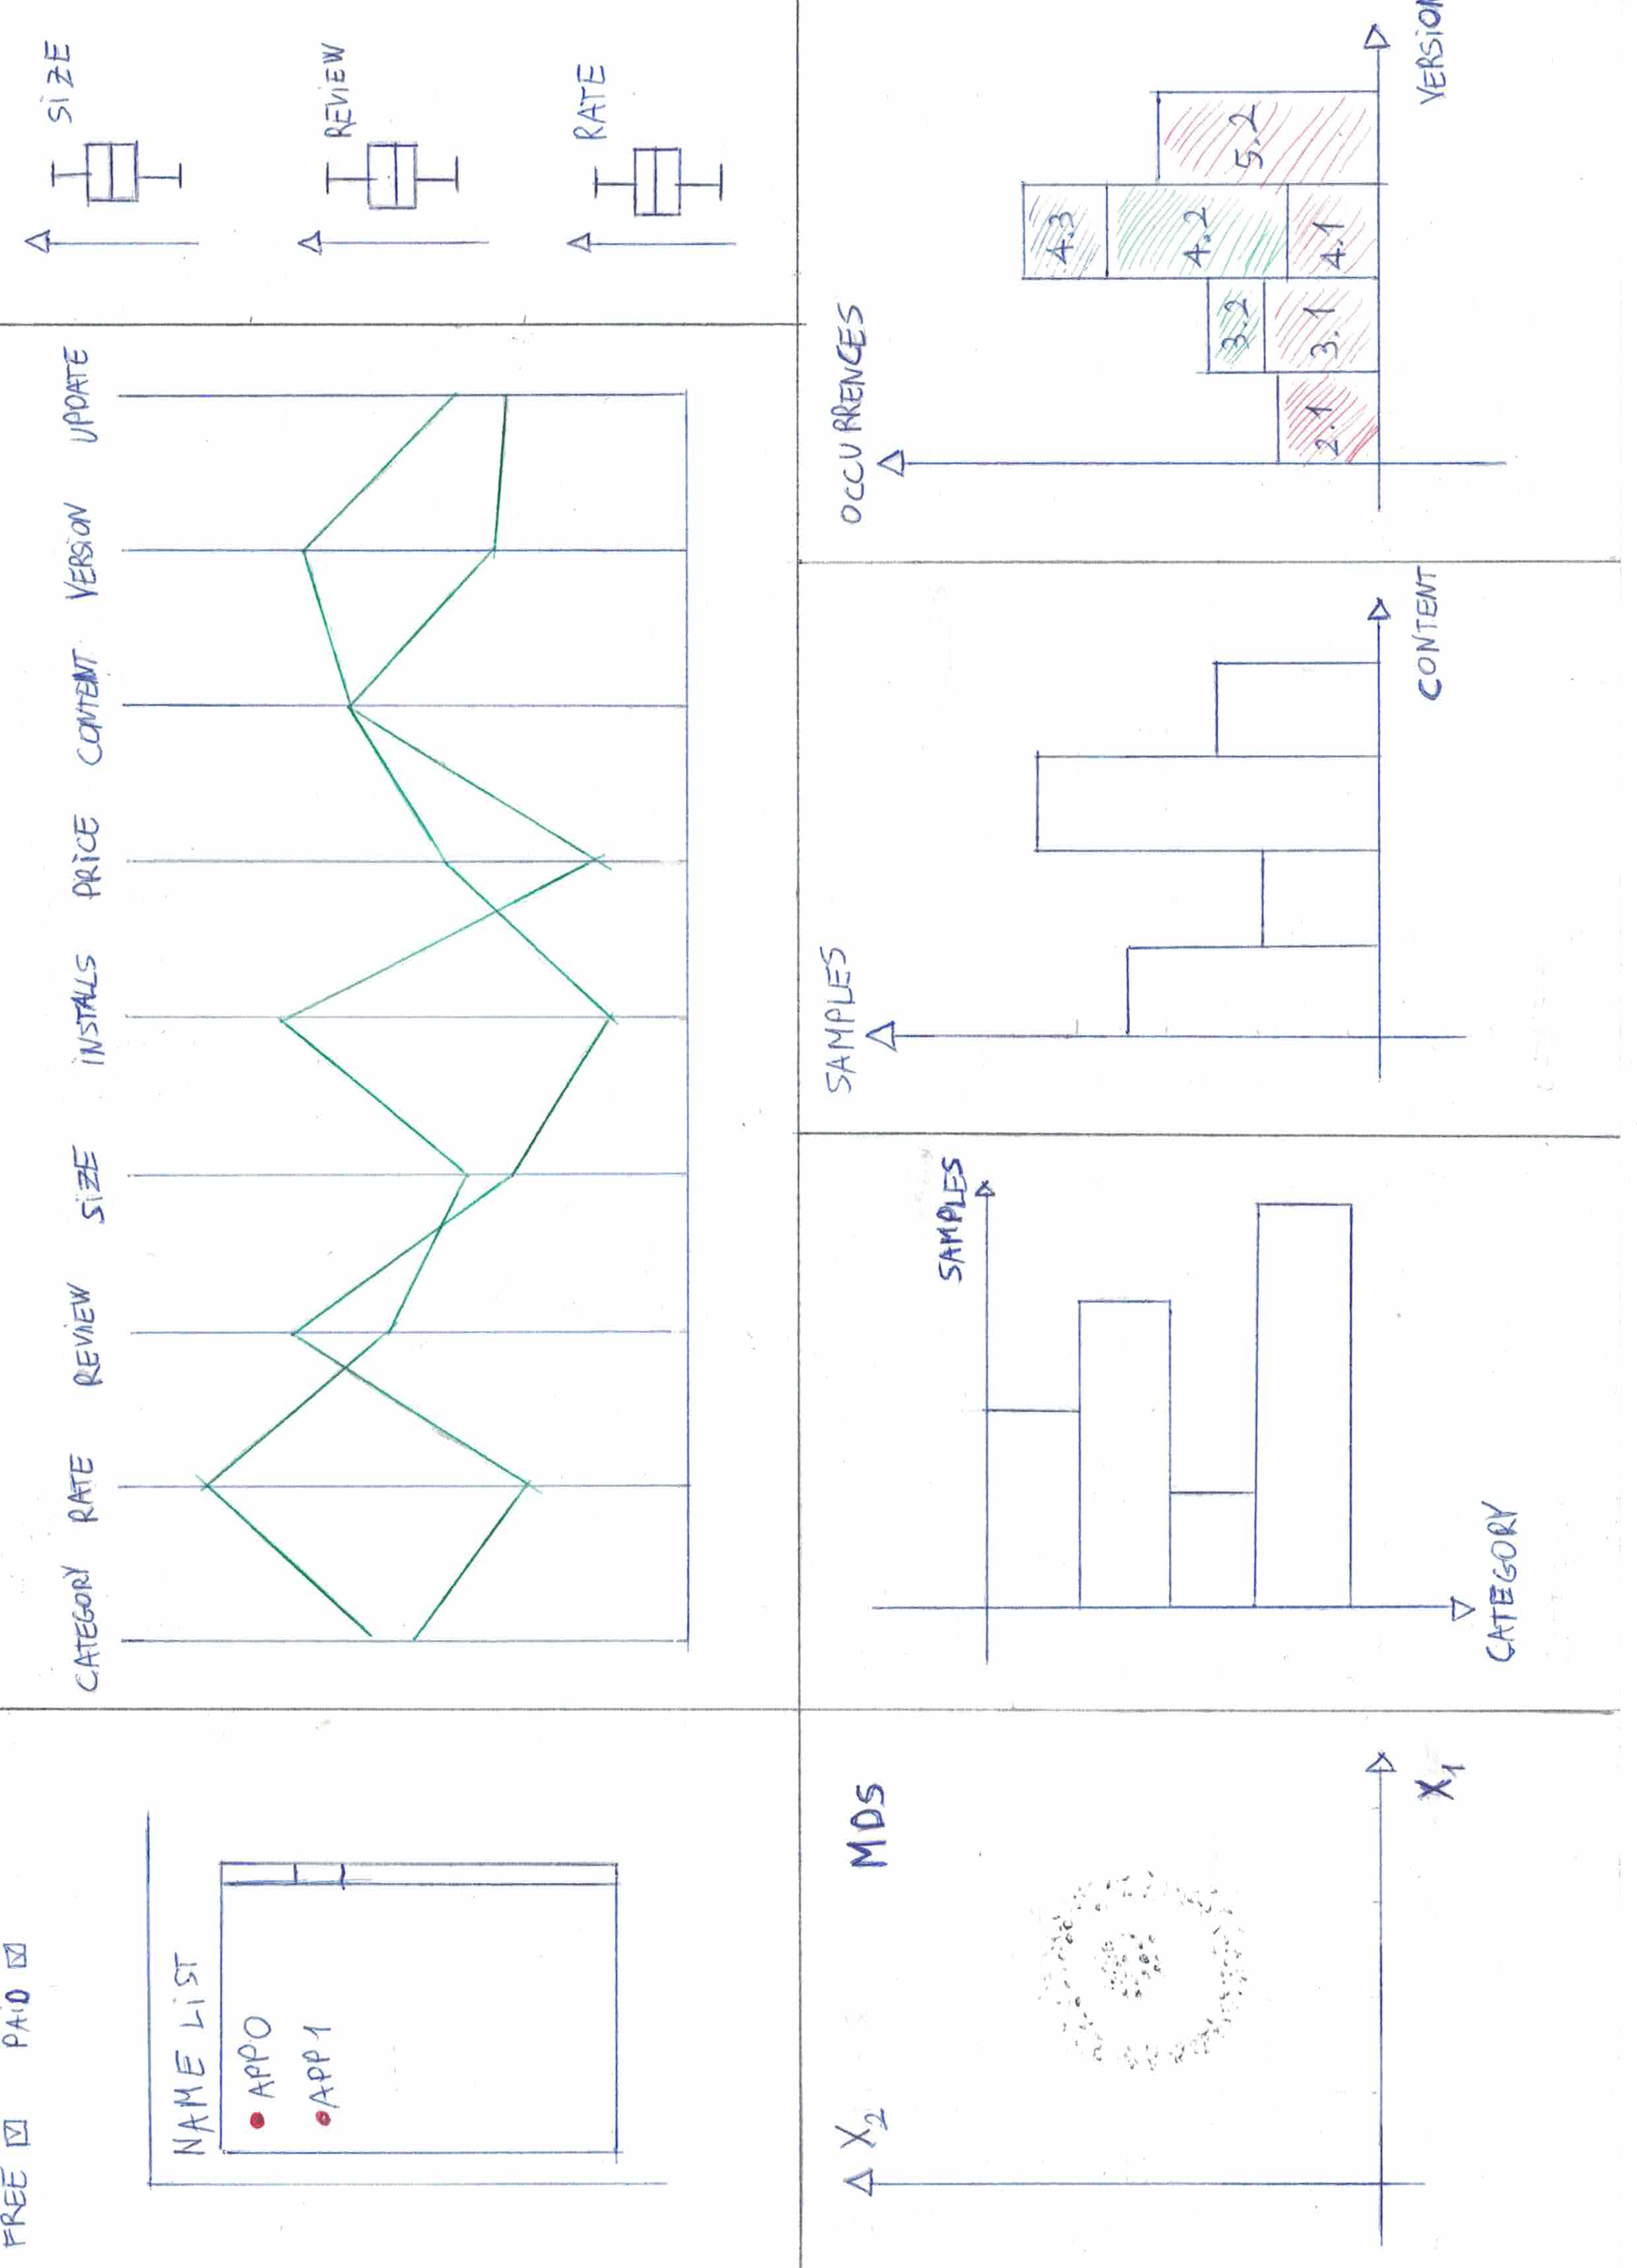
\includegraphics[width=\textwidth, angle=180]{mockup.png}
\end{document}
